% arara: pdflatex: { shell: yes }
% arara: pythontex: {verbose: yes, rerun: modified }
% arara: pdflatex: { shell: yes }
% arara: clean: {extensions: [blg, fls, log, out, pytxcode, rel] }

\documentclass[study-guide-sol]{subfiles}
\externaldocument{study-guide}

\opt{solutionfiles,check}{
\Opensolutionfile{hint}
\Opensolutionfile{ans}
}

\begin{document}

%\refcheckxrdoc[a]{memoryless_excursions}

\section{Exercises on 2D integration}
\label{sec:exerc-2d-integr}

Here is some extra material for you practice on 2D integration, indicators and 2D LOTUS. These exercises are old exam questions, hence quite a bit harder than the above.  They form important training.

\begin{exercise}
Let $X$ and $Y$ be continuous random variables. Furthermore, $F(x,y)$ is the joint cumulative distribution function of $X$ and $Y$. This function has the following properties.
\begin{align*}\
    \begin{array}{lll}
        1. &F(x,y) = \dfrac{1}{8}(x-1)^2(y-2) & \text{for } 1< x<3 \text{ and  } 2< y< 4,\vspace{0.2cm}\\
        2. &\dfrac{\partial F(x,y)}{\partial x}=0& \text{for } x\notin (1,3),\vspace{0.2cm}\\
        3. &\dfrac{\partial F(x,y)}{\partial y}=0&\text{for } y\notin (2, 4).
    \end{array}
\end{align*}
Use these properties to answer the following questions.
\begin{enumerate}
\item  What is $F(2,5)$?
\item  Determine the joint probability density function of $X$ and $Y$.
\item  Determine $\text{P}(2<X<3,\, 2<Y<4)$.
\item  Determine the joint probability $\text{P}(Y<2X,\, 2X+Y>6)$. Clearly draw the area over which you integrate.
\end{enumerate}
\begin{solution}
a.  \begin{align*}
                F(2,5) = P(X\leq 2,Y\leq 5) = P(X\leq 2,Y\leq 4) = F(2,4) = \frac{1}{4}
    \end{align*}
    The second step is valid since the cumulative distribution function does not change by changing $y$ from 5 to 4 thanks to property 3.

b.             To obtain the joint pdf, use that $f_{X,Y}(x,y) = \dfrac{\partial^2}{\partial y\partial x}F(x,y) = \dfrac{\partial}{\partial y}\left(\dfrac{\partial}{\partial x} F(x,y)\right)$.\\
            Since
            $\dfrac{\partial}{\partial x} F(x,y) = \dfrac{1}{4}(x-1)(y-2)$ for $1< x < 3$, and $\dfrac{\partial}{\partial x} F(x,y) = 0$ for other values of $x$, we have that
            \begin{align*}
                f_{X,Y}(x,y) = \begin{cases}
                    \dfrac{1}{4}(x-1), & \mbox{for } 1<x<3 \mbox{ and } 2<y<4,\\
                    0, & \mbox{elsewhere}.
                \end{cases}
            \end{align*}

c.            The simplest way of solving this question is by writing
            \begin{align*}
                P(2<X<3,\, 2<Y<4) &= F(3,4) - F(2,4) - F(3,2) + F(2,2) \\
                &= 1 - \frac{1}{4} -0 + 0 = \frac{3}{4}.
            \end{align*}
            Alternatively, one can integrate over the pdf from (b) to obtain the same result:
            \begin{align*}
                P(2<X<3,\, 2<Y<4) &= \int_2^3\int_2^4f(x,y)\text{d}y\text{d}x\\
                &=\frac{1}{4}\int_2^3\left.(x-1)y\right|_{y=2}^{y=4}\text{d}x\\
                &=\frac{1}{4}\left(\left.x^2-2x\right|_2^3\right) = \frac{1}{4}\left(9-6-4+4\right) = \frac{3}{4}.
            \end{align*}


d.     First, draw the integration area:
            \begin{center}
                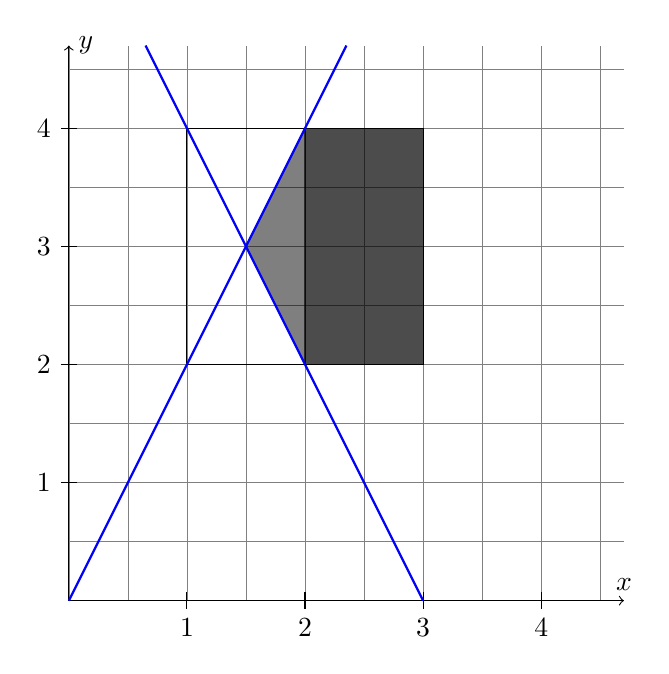
\begin{tikzpicture}[scale = 1.5]

                    \draw (1.05cm,2pt) node[above]{};
                    %  {$\displaystyle\int_0^{3/2} \!\!x^2\mathrm{d}x$};

                    \draw[style=help lines, step = 0.5] (0,0) grid (4.7,4.7);
                    % [step=0.25cm]      (1,2) grid +(1,1);

                    \draw[->] (0,0) -- (0,4.7) node[right] {$y$};
                    \draw[->] (0,0) -- (4.7,0) node[above] {$x$};
                    \foreach \x/\xtext in {1/1, 2/2, 3/3, 4/4}
                    \draw[shift={(\x,0)}] (0pt,2pt) -- (0pt,-2pt) node[below] {$\xtext$};

                    \foreach \y/\ytext in {1/1, 2/2, 3/3, 4/4}
                    \draw[shift={(0,\y)}] (2pt,0pt) -- (-2pt,0pt) node[left] {$\ytext$};

                    \draw[fill=black, fill opacity = 0]  (1,2) -- (1,4) -- (3,4) -- (3,2) -- cycle;
                    \draw[fill=black, fill opacity = 0.5]  (1.5,3) -- (2,4) -- (2,2);
                    \fill[black, fill opacity = 0.7] (2,4) -- (3,4) -- (3,2) -- (2,2);
                    \draw[domain=0.65:3,smooth,variable=\x,blue, thick] plot ({\x},{6-2*\x});
                    \draw[domain=0:2.35,smooth,variable=\x,blue, thick] plot ({\x},{2*\x});
                \end{tikzpicture}
            \end{center}
            The domain on which the density is non-zero, is the complete shaded area. The downward-sloping line represents $2x+y=6$ and the upward-sloping line is $y=2x$.

            We already know the integral over the dark shaded area from the previous subquestion. What remains is the lighter shaded triangular part on the left side.\\

                First, we need to calculate the intersection of the two curves, which can be found by solving $6-2x = 2x$, which gives $x= \frac{3}{2}$, and consequently $y = 3$.\\

            The integral of the triangular part of the dark shaded region is
            \begin{align*}
                \int_{3/2}^{2}\int_{6-2x}^{2x}\frac{1}{4}(x-1)dydx &= \int_{3/2}^{2}\left.\frac{1}{4}(x-1)y\right|_{6-2x}^{2x}dx\\
                &=\frac{1}{4}\int_{3/2}^{2}(x-1)2x-(x-1)(6-2x)dx\\
                &=\frac{1}{4}\int_{3/2}^{2}(x-1)(4x-6)dx\\
                &=\frac{1}{4}[\frac{4}{3}x^3-5x^2+6x]^{2}_{3/2}\\
                &=\dfrac{5}{48}\approx 0.1042\\
            \end{align*}
            Finally, the joint probability asked for in the question is given by
            $$P(Y<2X, 2X+Y>6) = \dfrac{5}{48}+\frac{3}{4} = \dfrac{41}{48}\approx 0.8542$$


\end{solution}
\end{exercise}

\begin{exercise}
 Suppose $X$ and $V$ are independent, $X\sim \text{Expo}(\lambda)$ and $V\sim \text{Expo}(\mu)$. Define the ratio $R=X/V$ and derive the cumulative distribution function (CDF) of $R$. Provide at least two checks on the CDF to make sure that your result is indeed a valid CDF.
    Note: There is no need to derive the probability density function (PDF) of $R$.
\begin{solution}
            For $r\geq 0$, we have
            \begin{align*}
                F_{R}(r)& = P(R\leq r) \\
                &= P(X\leq Vr)\\
                & = \int_{-\infty}^{\infty}\int_{-\infty}^{vr}f_{X,V}(x,v)dxdv\\
                & = \lambda\mu \int_{0}^{\infty}\int_{0}^{vr}e^{-\lambda x}e^{-\mu{v}}dxdv\\
                & = \lambda\mu\int_{0}^{\infty}e^{-\mu v}\left[-\frac{1}{\lambda}e^{-\lambda x}\right]_{0}^{vr}dv\\
                & = -\mu \int_{0}^{\infty}e^{-\mu v}(e^{-\lambda vr}-1)dv\\
                & = -\mu\left[-\frac{1}{\mu +\lambda r}e^{-(\mu+\lambda r)v}+\frac{1}{\mu}e^{-\mu v}\right]_{0}^{\infty}\\
                & = -\mu\left[\frac{1}{\mu+\lambda r}-\frac{1}{\mu}\right]\\
                & = \frac{\lambda r}{\mu+\lambda r},
            \end{align*}
            while $F_{R}(r)=0$ when $r<0$ since both $X$ and $V$ are nonnegative.

            We see that (1) $F_{R}(-\infty)=0$, (2) $F_{R}(\infty)=1$, and (3) $F_{R}(r)$ is monotonically increasing in $r$, so $F_{R}(r)$ satisfies the conditions for being a valid CDF.
\end{solution}
\end{exercise}


\begin{exercise}
 Consider the following joint density function
\begin{align*}
    f_{X,Y}(x,y) = \left\{\begin{array}{ll}
        cxy & \text{ for } 0\leq x<\frac{1}{2} \text{ and } 0\leq y\leq x,\\
        cxy & \text{ for } \frac{1}{2}\leq x\leq 1 \text{ and } 0\leq y\leq 1-x,\\
        0 & \text{otherwise.}
    \end{array}\right.
\end{align*}
\begin{enumerate}
\item  What is the correct value of the constant $c$?
\item Derive the conditional probability density function $f_{X|Y}(x|y)$. Verify that your result is indeed a valid density function.
\end{enumerate}

 \begin{solution}
a.         We integrate $f_{X,Y}(x,y)$ over its domain
        \begin{align*}
            &\int_{0}^{1/2}\int_{0}^{x}cxydydx + \int_{1/2}^{1}\int_{0}^{1-x}cxydydx\\
            = &c\left[\frac{1}{2}\int_{0}^{1/2}x^3dx + \frac{1}{2}\int_{1/2}^{1}x(1-x)^2dx\right]\\
            =&\frac{1}{2}c\left\{\left[\frac{1}{4}x^4\right]^{1/2}_{0} + \left[\frac{1}{2}x^2-\frac{2}{3}x^{3}+\frac{1}{4}x^{4}\right]^{1}_{1/2}\right\}\\
            & = \frac{1}{2}c\left\{\frac{1}{4}\frac{1}{16} + \frac{1}{2}-\frac{2}{3}+\frac{1}{4}-\frac{1}{2}\frac{1}{4} + \frac{2}{3}\frac{1}{8} - \frac{1}{4}\frac{1}{16}\right\}\\
            & = \frac{1}{2}c\frac{12-16+6-3+2}{24}\\
            & = \frac{c}{48}
        \end{align*}
        Since this integral should equal 1, $c = 48$. \newline\newline
        \textbf{Alternative} Rewrite the probability density function to
        \begin{align*}
            f_{X,Y}(x,y) = \left\{\begin{array}{ll}
                cxy & 0\leq y\leq \frac{1}{2},\quad y\leq x\leq 1-y\\
                0 & \text{otherwise}
            \end{array}\right.
        \end{align*}
        Then,
        \begin{align*}
            \int_{0}^{1/2}\int_{y}^{1-y}cxydxdy& = c\int_{0}^{1/2}y\frac{1}{2}\left((1-y)^2-y^2\right)\\
            & = \frac{1}{2}c\int_{0}^{1/2}\left( y-2y^2\right)dy\\
            &=\frac{1}{2}c\left[\frac{1}{2}y^2-\frac{2}{3}y^3\right]_{0}^{1/2}\\
            &=\frac{1}{2}c\left[ \frac{1}{8}-\frac{2}{3}\frac{1}{8}\right]
            =\frac{c}{48}
        \end{align*}
        Since this integral should equal 1, $c = 48$.


 b.
        The conditional density function is given by
        \begin{align*}
            f_{X|Y}(x|y) = \frac{f_{X,Y}(x,y)}{f_{Y}(y)}
        \end{align*}
        We first need the marginal density of $Y$.
        \begin{align*}
            f_{Y}(y)& = 48\int_{y}^{1-y}xydx\\
            & = 48y\left[\frac{1}{2}(1-y)^2-\frac{1}{2}y^2\right]\\
            &=24y\left[1-2y+y^2-y^2\right]\\
            &=24y(1-2y)\quad\text{for } 0\leq y\leq \frac{1}{2}
        \end{align*}
        and $f_{Y}(y)=0$ otherwise.
        \hrule\vspace{0.2cm}
        \textit{Not required}: We can check that this is a valid density function:
        \begin{align*}
            \int_{0}^{1/2}24y(1-2y)dy &= 24\left[\frac{1}{2}y^2-\frac{2}{3}y^3\right]^{1/2}_{0}\\
            & = 24\left[\frac{1}{2}\frac{1}{4}-\frac{2}{3}\frac{1}{8}\right]^{1/2}_{0}\\
            &=1
        \end{align*}
        \hrule\vspace{0.2cm}

b. Now we can obtain the conditional density function
        \begin{align*}
            f_{X|Y}(x|y) &=\frac{f_{X,Y}(x,y)}{f_{Y}(y)}\\
            &= \frac{48xy}{24y(1-2y)} = \frac{2x}{1-2y} \quad \text{for } y\leq x\leq 1-y, \text{ and } 0\leq y<\frac{1}{2}
        \end{align*}
        and $f_{X|Y}(x|y)=0$ otherwise. \newline\newline
        This is a valid density function since $f(X|Y)(x|y)\geq 0$, and
        \begin{align*}
            \int_{y}^{1-y}f_{X|Y}(x|y)dx & = \frac{2}{1-2y}\left[\frac{1}{2}x^2\right]^{1-y}_{y}\\
            &=1
        \end{align*}
\end{solution}
\end{exercise}

\begin{exercise}
 Suppose the random variables $X$ and $Y$ have the joint probability density function
\begin{align*}
    f_{X,Y}(x,y) = \left\{\begin{array}{cl}
        2 & \text{if } 0\leq x< 1,\quad  |y|<\frac{1}{2}(1-x),\\
        0 & \text{otherwise}
    \end{array}\right.
\end{align*}

\begin{enumerate}
\item Calculate the marginal probability density functions $f_{X}(x)$ and $f_{Y}(y)$ and show that these are valid probability density functions.
\item Find the conditional expectation $\text{E}[X|Y=y]$. Provide at least one `sanity check' that shows that your answer makes intuitive sense.
    If you did not find an answer to (a), you can use that
    \begin{align*}
        f_{Y}(y) = \left\{\begin{array}{ll}
            2(1-2|y|)&\text{ if } -\frac{1}{2}< y<\frac{1}{2},\\
            0 & \text{ otherwise}.
        \end{array}\right.
    \end{align*}
\item Calculate the joint cumulative distribution function $F_{X,Y}(x,y)$ for $x=\frac{1}{2}$ and $y=3$.
\end{enumerate}


\begin{solution}
a.             The joint PDF is nonzero above the red-shaded area in the following graph. (draw, draw, draw!)
            \begin{center}
                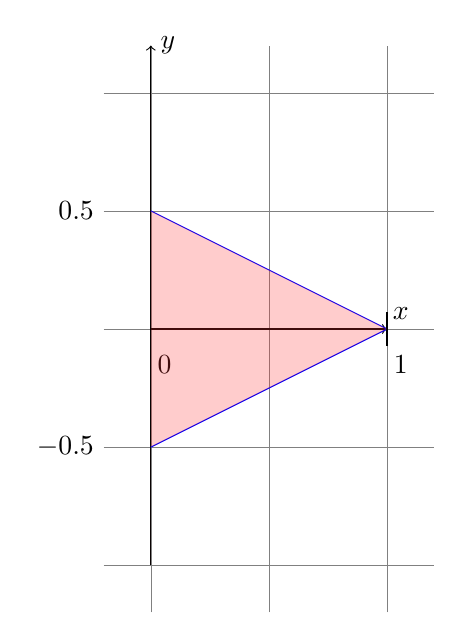
\begin{tikzpicture}[scale = 3]

                    \draw (1.05cm,2pt) node[above]{};
                    %  {$\displaystyle\int_0^{3/2} \!\!x^2\mathrm{d}x$};

                    \draw[style=help lines, step = 0.5] (-0.2,-1.2) grid (1.2,1.2);
                    % [step=0.25cm]      (1,2) grid +(1,1);

                    \draw[->] (0,-1) -- (0,1.2) node[right] {$y$};
                    \draw[->] (0,0) -- (1,0) node[above] {$\quad x$};
                    \draw[domain=(0):1,smooth,variable=\x,blue] plot ({\x},{0.5-0.5*\x});
                    \draw[domain=(0):1,smooth,variable=\x,blue] plot ({\x},{0.5*\x-0.5});
                    \foreach \x/\xtext in {0/0, 1/1}
                    \draw[shift={(\x,0)}] (0pt,2pt) -- (0pt,-2pt) node[below] {$\quad\xtext$};

                    \foreach \y/\ytext in {-0.5/-0.5,0.5/0.5}
                    \draw[shift={(-0.2,\y)}] node[left] {$\ytext$};

                    %		\draw[fill=red]  (0,11) -- (3,8) -- (3,4) -- (0,7) -- cycle;
                    %				\draw [dashed] (0,0.5) -- (0.75,0.5) node[right] {$\left(\frac{3}{4},\frac{1}{2}\right)$};
                    %				\draw [dashed] (0.75,0)-- (0.75,0.5);
                    %				\fill[red!20, nearly transparent]
                    %				[domain=0:0.5,smooth,variable=\x] (0,1) -- plot
                    %				({\x},{\x}) -- (1,1);
                    \fill[red!80, nearly transparent]
                    [domain=0:1,smooth,variable=\x] (0,-1) -- plot ({\x},{0.5*(\x-1)}) -- (0,0);
                    \fill[red!80, nearly transparent]
                    [domain=0:1,smooth,variable=\x] (0,1) -- plot ({\x},{0.5*(1-\x)}) -- (0,0);
                    % \fill[gray!20] (0,11) -- (0,12) -- (3,12) -- (3,8) -- cycle; %without transparency
                \end{tikzpicture}
            \end{center}

For the PDF  for $Y$,             using the graph above,
            \begin{align*}
                f_{Y}(y) &= \int_{-\infty}^{\infty}f_{X,Y}(x,y)dx\\
                & = \int_{0}^{1-2|y|}2dx\\
                & = 2(1-2|y|)\quad\text{for } -1/2< y< 1/2,
            \end{align*}
            and 0 otherwise.
            Since $-1/2< y< 1/2$, we have $f_{Y}(y)\geq 0$. Also,
            \begin{align*}
                \int_{-\infty}^{\infty}f_{Y}(y)dy &= \int_{-1/2}^{1/2}2(1-2|y|)dy\\
                &=2\int_{0}^{1/2}(1-2y)dy + 2\int_{-1/2}^{0}(1+2y)dy\\
                &=2\left(\frac{1}{2}-\frac{1}{4} +\frac{1}{2}-\frac{1}{4}\right) = 1.
            \end{align*}

Probability density function for $X$.
            \begin{align*}
                f_{X}(x) & = \int_{-\infty}^{\infty}f_{X,Y}dy\\
                & = \int_{-\frac{1}{2}(1-x)}^{\frac{1}{2}(1-x)}2dy\\
                & = 2(1-x)\quad\text{for } 0\leq x< 1,
            \end{align*}
            and 0 otherwise.
            We have $f_{X}(x)\geq 0$, and also
            \begin{align*}
                \int_{-\infty}^{\infty}f_{X}(x)dx &= \int_{0}^{1}2(1-x)dx\\
                &=2\left[x-\frac{1}{2}x^2\right]_{0}^{1}\\
                & = 2\left(1-\frac{1}{2}\right) = 1.
            \end{align*}
            Since $-1/2< y< 1/2$, we have $f_{Y}(y)\geq 0$. Also,
            \begin{align*}
                \int_{-\infty}^{\infty}f_{Y}(y)dy &= \int_{-1/2}^{1/2}2(1-2|y|)dy\\
                &=2\int_{0}^{1/2}(1-2y)dy + 2\int_{-1/2}^{0}(1+2y)dy\\
                &=2\left(\frac{1}{2}-\frac{1}{4} +\frac{1}{2}-\frac{1}{4}\right) = 1.
            \end{align*}

Probability density function for $X$.
            \begin{align*}
                f_{X}(x) & = \int_{-\infty}^{\infty}f_{X,Y}dy\\
                & = \int_{-\frac{1}{2}(1+x)}^{\frac{1}{2}(1+x)}2dy\\
                & = 2(1+x)\quad\text{for } -1< x\leq 0,
            \end{align*}
            and 0 otherwise.
            We have $f_{X}(x)\geq 0$, and also
            \begin{align*}
                \int_{-\infty}^{\infty}f_{X}(x)dx &= \int_{-1}^{0}2(1+x)dx\\
                &=2\left[x+\frac{1}{2}x^2\right]_{-1}^{0}\\
                & = 2\left(1-\frac{1}{2}\right) = 1.
            \end{align*}

b.
            Using the definition of a conditional probability density function, we have
            \begin{align*}
                f_{X|Y}(x|y) = \frac{f_{X,Y}(x,y)}{f_{Y}(y)}=\frac{1}{1-2|y|}\quad\text{for }-\frac{1}{2}<y<\frac{1}{2}, 0<x<1-2|y|
            \end{align*}
            and $0$ otherwise.


            The required expected value is (bounds are crucial!)
            \begin{align*}
                \text{E}[X|Y=y] = \int_{0}^{1-2|y|}\frac{x}{1-2|y|}dx = \frac{1}{2}(1-2|y|).
            \end{align*}
            If $y=-1/2$ or $y=1/2$, we find $\text{E}[X|Y=y]=0$, which makes sense based on the figure above. Similarly, if $y=0$, we find $\text{E}[X|Y=y] = 1/2$ since the density of $x$ is uniform over $[0,1]$.


            The point ($\frac{1}{2},3$) is located as in the picture below. We need to integrate $f_{X,Y}(x,y)$ over the entire area on the lower left side of this point. It is crucial to realize that the joint PDF is only nonzero in the red shaded area. Moreover, it's very helpful that the PDF has a constant value of 2 above this area.
            So we just need to calculate the the area of the red shape in the following graph and multiply this by 2.
            \begin{center}
                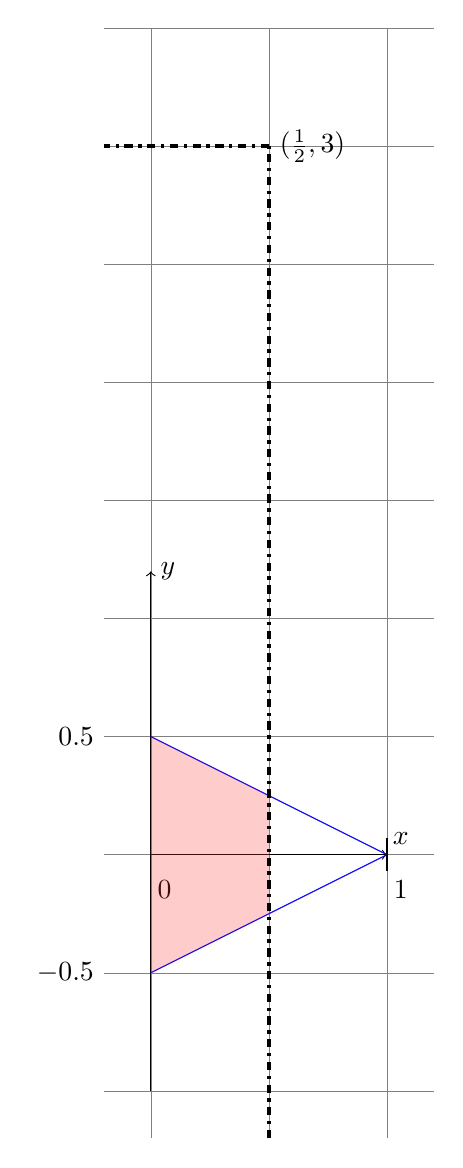
\begin{tikzpicture}[scale = 3]
                    \draw (1.05cm,2pt) node[above]{};
                    %  {$\displaystyle\int_0^{3/2} \!\!x^2\mathrm{d}x$};

                    \draw[style=help lines, step = 0.5] (-0.2,-1.2) grid (1.2,3.5);
                    % [step=0.25cm]      (1,2) grid +(1,1);

                    \draw[->] (0,-1) -- (0,1.2) node[right] {$y$};
                    \draw[->] (0,0) -- (1,0) node[above] {$\quad x$};
                    \draw[domain=(0):1,smooth,variable=\x,blue] plot ({\x},{0.5*(1-\x)});
                    \draw[domain=(0):1,smooth,variable=\x,blue] plot ({\x},{0.5*(\x-1)});
                    \foreach \x/\xtext in {0/0, 1/1}
                    \draw[shift={(\x,0)}] (0pt,2pt) -- (0pt,-2pt) node[below] {$\quad\xtext$};

                    \foreach \y/\ytext in {-0.5/-0.5, 0.5/0.5}
                    \draw[shift={(-0.2,\y)}] node[left] {$\ytext$};

                    \fill[red!80, nearly transparent]
                    [domain=0:1,smooth,variable=\x] (0.5,-0.25) -- (0.5,0.25) -- plot ({\x},{0.5*(1-\x)}) -- (0,0.5) -- (0,-0.5) -- plot ({\x},{0.5*(\x-1)});
                    \draw [very thick, dash dot] (0.5,-1.2) -- (0.5,3) node[right] {$(\frac{1}{2},3)$};
                    \draw [very thick, dash dot] (0.5,3) -- (-0.2,3);
                    % \fill[gray!20] (0,11) -- (0,12) -- (3,12) -- (3,8) -- cycle; %without transparency
                \end{tikzpicture}
            \end{center}
            The dash dotted line intersects the line $y = \frac{1}{2}(1-x)$ at $x=\frac{1}{2}$, so $y=\frac{1}{4}$. The line intersects $y=-\frac{1}{2}(1-x)$ at $x=\frac{1}{2}$, so $y=-\frac{1}{4}$.
            The whole area of the triangle is $\frac{1}{2}$. The area \textit{not} in red is $\frac{1}{2}\cdot(\frac{1}{4}-(-\frac{1}{4}))\cdot (1-\frac{1}{2}) = \frac{1}{8}$. So\
            \begin{equation*}
                F_{X,Y}\left(\frac{1}{2},3\right) =2\left(\frac{1}{2}-\frac{1}{8}\right)=\frac{3}{4}.
            \end{equation*}
\end{solution}
\end{exercise}


\begin{exercise}
Suppose the joint probability density function of $X$ and $Y$ is given by
\begin{equation*}
    f_{X,Y}(x,y) = \frac{c}{1-x}, \quad 0<x+y<1, \quad x>0, \quad y>0
\end{equation*}
and $f_{X,Y}(x,y)=0$ otherwise.
\begin{enumerate}
\item
For what value of the constant $c$ is $f_{X,Y}(x,y)$ a joint probability density function?
\item     What is the probability that $X+Y>\frac{1}{2}$?
\item     What is the probability that both $X$ and $Y$ are smaller than $\frac{1}{2}$ given that $X+Y>\frac{1}{2}$?
\end{enumerate}
\begin{solution}
a.        $f_{X,Y}(x,y)$ is a joint probability density function if
        \begin{enumerate}
            \item If $f_{X,Y}(x,y)$ satisfies
            \begin{align*}
                \int_{-\infty}^{\infty}\int_{-\infty}^{\infty}f_{X,Y}(x,y)dxdy = 1
            \end{align*}
            \item $f_{X,Y}(x,y)\geq 0$ for all $x$ and $y$.
        \end{enumerate}

        We have
        \begin{align*}
            \int_{-\infty}^{\infty}\int_{-\infty}^{\infty}f_{X,Y}(x,y)dydx& = \int_{0}^{1}\int_{0}^{1-x} \frac{c}{1-x}dydx \\
            &= c\int_{0}^{1}\frac{1-x}{1-x}dx = 1
        \end{align*}
        So to satisfy condition (1), we need to set $c=1$. \newline
        Check Condition (2): $f_{X,Y}(x,y)\geq 0$ for all $x,y$. \newline
        For $0<x<1$, $f_{X,Y}(x,y)> 0$. Outside of this interval $f_{X,Y}(x,y)=0$. So, we have that $f_{X,Y}(x,y)\geq 0$ for all $x,y$.\newline
        %	\textit{Correct integral limits, but calculation error leading to the wrong constant: -1 point.\newline
        %		 Forgetting to check whether $f_{X,Y}(x,y)\geq 0$, do not subtract points.}

b.         The following graph is used for questions $b$ and $c$.
        \begin{center}
            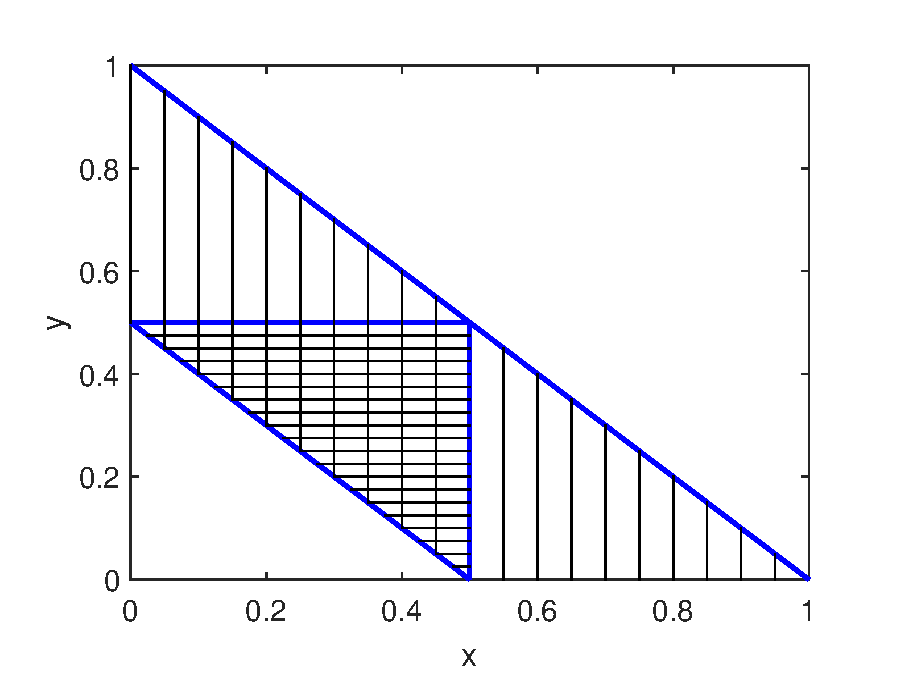
\includegraphics[width = 0.7\textwidth]{figures/pie.eps}
        \end{center}
        To obtain $P(X+Y>1/2)$, we need to integrate $f_{X,Y}$ over the vertically hatched area. We do this by integrating over the larger triangle defined by $x+y<1$, and then subtract the white triangle in the lower left corner defined by $x+y<\frac{1}{2}$.
        \begin{align*}
            P\left(X+Y>\frac{1}{2}\right) &= \int_{0}^{1}\int_{0}^{1-x}\frac{1}{1-x}dydx - \int_{0}^{1/2}\int_{0}^{1/2-x}\frac{1}{1-x}dydx\\
            & = 1-\int_{0}^{1/2}\frac{1/2-x}{1-x}dx\\
            & = 1-\int_{0}^{1/2}\left(1-\frac{1}{2}\frac{1}{1-x}\right)dx\\
            & = 1-\frac{1}{2} + \frac{1}{2}\int_{0}^{1/2}\frac{1}{1-x}dx\\
            & = \frac{1}{2}+\frac{1}{2}\left[-\ln(1-x)\right]^{1/2}_{0}\\
            & = \frac{1}{2}-\frac{1}{2}\ln\left(\frac{1}{2}\right)=0.8466
        \end{align*}
        %	\textit{Integrating over the wrong triangle: -2 points.\\
        %		Minor calculation errors: -1 point.\\
        %		Major calculation errors: -2 points.}


c.         Using the definition of conditional probability
        \begin{align*}
            P\left(X<\frac{1}{2},Y<\frac{1}{2}\left|X+Y>\frac{1}{2}\right.\right) = \frac{P\left(X<\frac{1}{2},Y<\frac{1}{2},X+Y>\frac{1}{2}\right)}{P\left(X+Y>\frac{1}{2}\right)}
        \end{align*}
        The integral in the numerator is the integral over the horizontally hatched triangle. Easiest is to first integrate over the square $[0,1/2]\times[0,1/2]$ and then subtract the lower white triangle, which we have already calculated in the previous question to be $\frac{1}{2}+\frac{1}{2}\ln\left(\frac{1}{2}\right)$.
        \begin{align*}
            \int_{0}^{1/2}\int_{0}^{1/2}\frac{1}{1-x}dydx & = \frac{1}{2}\int_{0}^{1/2}\frac{1}{1-x}dx\\
            & = \frac{1}{2}\left[-\ln(1-x)\right]^{1/2}_{0}\\
            & = -\frac{1}{2}\ln\left(\frac{1}{2}\right)
        \end{align*}
        Subtracting the lower triangle from the square, we see that the integral over the horizontally hatched triangle equals
        \begin{align*}
            -\frac{1}{2}\ln\left(\frac{1}{2}\right) - \frac{1}{2}-\frac{1}{2}\ln\left(\frac{1}{2}\right)=-\frac{1}{2}-\ln\left(\frac{1}{2}\right)
        \end{align*}
        We can then calculate
        \begin{align*}
            P\left(X<\frac{1}{2},Y<\frac{1}{2}|X+Y>\frac{1}{2}\right)=\frac{-\frac{1}{2}-\ln\left(\frac{1}{2}\right)}{\frac{1}{2}-\frac{1}{2}\ln\left(\frac{1}{2}\right)}\approx 0.23
        \end{align*}
        %	\textit{Integrating over the wrong triangle: -2 points.\\
        %		Minor calculation errors: -1 point.\\
        %		Major calculation errors: -2 points.}
\end{solution}
\end{exercise}


\begin{exercise}
 $X$ and $Y$ be random variables with joint probability density function
$$f_{X,Y}(x,y) = \begin{cases}
    \frac{3}{16}xy^2, & 0\le x\le c\mbox{ and } 0\le y\le c,\\
    0, & \mbox{elsewhere}
\end{cases}$$ where $c>0$ is a real number.
\begin{enumerate}
\item  Show that $c = 2$.
\item Show that $P(X+Y>2) = \frac{9}{10}$. Start by making a clear sketch of the area in the $(x,y)$-plane over which you take the required integral.
\item Calculate the conditional probability $P\left(\left.Y<X^2\right|X+Y<2\right)$.
\end{enumerate}
\begin{solution}
a.            Since $f_{XY}(x,y)$ is a joint probability density function, we should have\\
            1. $f_{X,Y}(x,y)\geq 0$. This is satisfied since $x,y\geq 0$. % \hfill \textbf{(1 point)}\\
            2.  $$\int_{-\infty}^{\infty}\int_{-\infty}^{\infty}f_{XY}(x,y)\text{d}x\text{d}y = 1,$$.
            We can calculate the integral as follows.
            \begin{alignat*}{3}
                \int_{-\infty}^{\infty}\int_{-\infty}^{\infty}f_{XY}(x,y)\text{d}x\text{d}y = 1\iff && \frac{3}{16}\int_{0}^{c}\int_{0}^{c}xy^2\text{d}x\text{d}y &= 1\\
                \iff && \frac{3}{32}\int_{0}^{c}\left(\left.x^2y^2\right|_0^c\right)\text{d}y &= 1\\
                \iff && \frac{3c^2}{32}\int_{0}^{c}y^2\text{d}y &= 1\\
                \iff && \left.\frac{3c^2}{96}y^3\right|_0^c &= 1\\
                \iff && 3c^5 &= 96
                \iff  c = 2 %\tag*{(\textbf{4 points})}
            \end{alignat*}

b. First, draw the area over which the integral is taken. %\hfill (\textbf{2 points})
            \begin{center}
                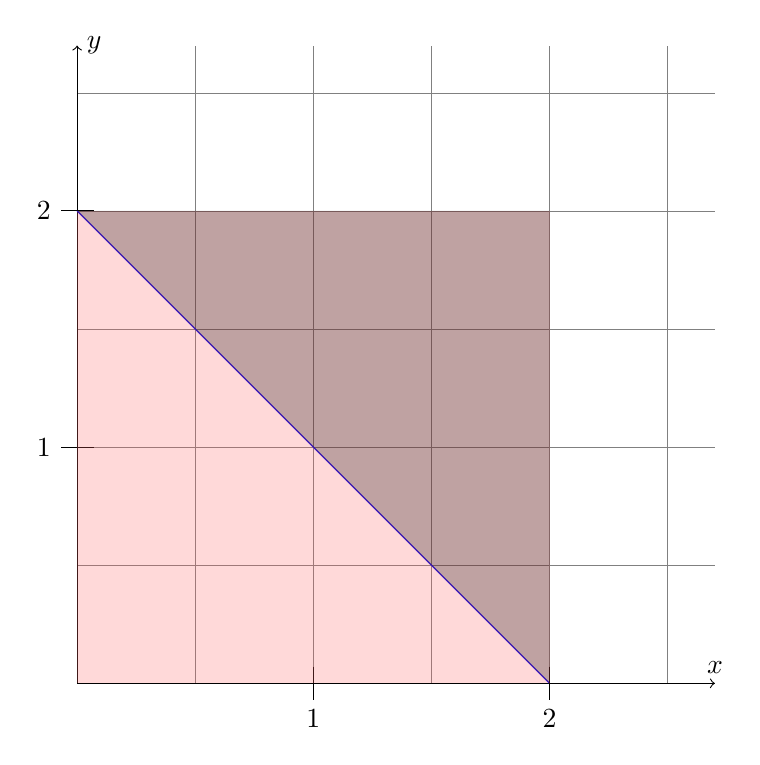
\begin{tikzpicture}[scale = 3]

                    \draw (1.05cm,2pt) node[above]{};
                    %  {$\displaystyle\int_0^{3/2} \!\!x^2\mathrm{d}x$};

                    \draw[style=help lines, step = 0.5] (0,0) grid (2.7,2.7);
                    % [step=0.25cm]      (1,2) grid +(1,1);

                    \draw[->] (0,0) -- (0,2.7) node[right] {$y$};
                    \draw[->] (0,0) -- (2.7,0) node[above] {$x$};
                    \draw[domain=(0):2,smooth,variable=\x,blue] plot ({\x},{2-\x});
                    \foreach \x/\xtext in {1/1, 2/2}
                    \draw[shift={(\x,0)}] (0pt,2pt) -- (0pt,-2pt) node[below] {$\xtext$};

                    \foreach \y/\ytext in {1/1, 2/2}
                    \draw[shift={(0,\y)}] (2pt,0pt) -- (-2pt,0pt) node[left] {$\ytext$};

                    %		\draw[fill=red]  (0,11) -- (3,8) -- (3,4) -- (0,7) -- cycle;
                    \fill[red!60, nearly transparent] (0,2) -- (2,2) -- (2,0) -- (0,0) -- cycle;
                    \fill[black, nearly transparent] [domain=0:2,smooth,variable=\x] plot ({\x},{2-\x}) -- (2,0) -- (2,2) -- (0,2);
                    % \fill[gray!20] (0,11) -- (0,12) -- (3,12) -- (3,8) -- cycle; %without transparency
                \end{tikzpicture}
            \end{center}

            We want to integrate over the darkest area. Hence, for every value of $y$, $x$ varies between $2-y$ and $2$. Hence, the required probability can be calculated as follows:\\
            \begin{minipage}[t]{0.45\textwidth}
                \textbf{Solution 1}
                \begin{align*}
                    &\quad P(X+Y>2)=\\
                    &= \int_{0}^{2}\int_{2-y}^{2}f_{X,Y}(x,y)\text{d}x\text{d}y\\
                    &= \frac{3}{16}\int_{0}^{2}\int_{2-y}^{2}xy^2\text{d}x\text{d}y\\
                    &= \frac{3}{32}\int_{0}^{2}\left(\left.x^2y^2\right|_{2-y}^2\right)\text{d}y\\
                    &= \frac{3}{32}\int_{0}^{2}(4y^2-(2-y)^2y^2)\text{d}y\\
                    &= \frac{3}{32}\int_{0}^{2}(4y^3-y^4)\text{d}y\\
                    &= \frac{3}{32}\left(\left.y^4-\frac{1}{5}y^5\right|_{0}^2\right)\\
                    &= \frac{3}{32}\left(16-\frac{32}{5}\right)\\
                    &= \frac{3}{2}-\frac{3}{5} = \frac{9}{10} %\tag*{(\textbf{3 points})}
                \end{align*}
            \end{minipage}
            \begin{minipage}[t]{0.45\textwidth}
                \textbf{Solution 2}
                \begin{align*}
                    &\quad P(X+Y>2)=\\
                    &= \int_{0}^{2}\int_{2-x}^{2}f_{X,Y}(x,y)\text{d}y\text{d}x\\
                    &= \frac{3}{16}\int_{0}^{2}\int_{2-x}^{2}xy^2\text{d}y\text{d}x\\
                    &= \frac{3}{16}\int_{0}^{2}\left(\left.\frac{1}{3}xy^3\right|_{2-x}^2\right)\text{d}x\\
                    &= \frac{1}{16}\int_{0}^{2}(8x-x(2-x)^3)\text{d}x\\
                    &= \frac{1}{16}\int_{0}^{2}(x^4+12x^2-6x^3)\text{d}x\\
                    &= \frac{1}{16}\left(\left.\frac{1}{5}x^5+4x^3-\frac{3}{2}x^4\right|_{0}^2\right)\\
                    &= \frac{1}{16}\left(\frac{32}{5}+32-24\right)\\
                    &= \frac{2}{5}+\frac{8}{16} = \frac{9}{10} %\tag*{(\textbf{3 points})}
                \end{align*}
            \end{minipage}
c. First, draw the area over which the integral is taken. % \hfill (\textbf{2 points})
            \begin{center}
                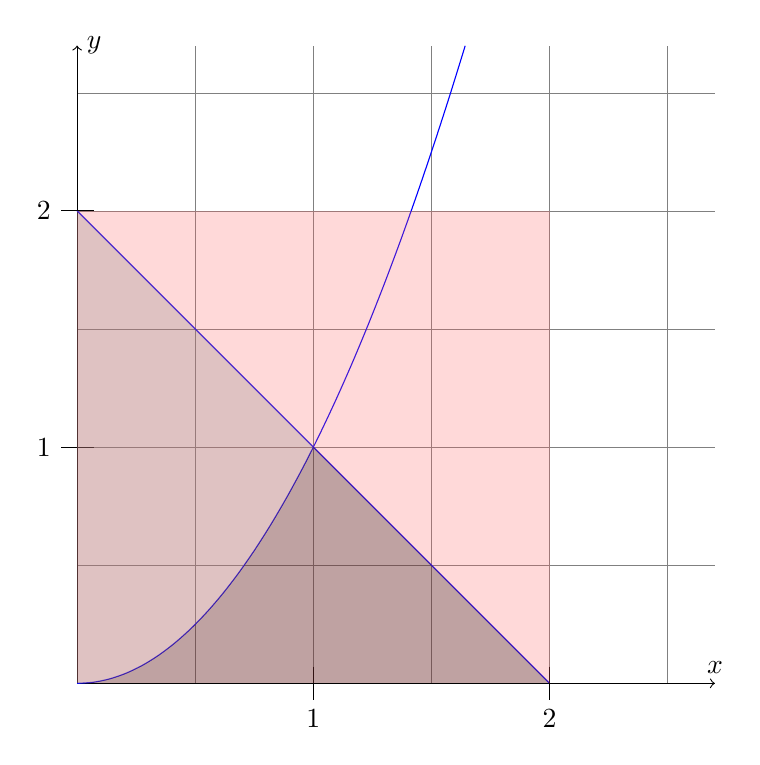
\begin{tikzpicture}[scale = 3]

                    \draw (1.05cm,2pt) node[above]{};
                    %  {$\displaystyle\int_0^{3/2} \!\!x^2\mathrm{d}x$};

                    \draw[style=help lines, step = 0.5] (0,0) grid (2.7,2.7);
                    % [step=0.25cm]      (1,2) grid +(1,1);

                    \draw[->] (0,0) -- (0,2.7) node[right] {$y$};
                    \draw[->] (0,0) -- (2.7,0) node[above] {$x$};
                    \draw[domain=0:2,smooth,variable=\x,blue] plot ({\x},{2-\x});
                    \draw[domain=0:sqrt(2.7),smooth,variable=\x,blue] plot ({\x},{\x*\x});
                    \foreach \x/\xtext in {1/1, 2/2}
                    \draw[shift={(\x,0)}] (0pt,2pt) -- (0pt,-2pt) node[below] {$\xtext$};

                    \foreach \y/\ytext in {1/1, 2/2}
                    \draw[shift={(0,\y)}] (2pt,0pt) -- (-2pt,0pt) node[left] {$\ytext$};

                    %		\draw[fill=red]  (0,11) -- (3,8) -- (3,4) -- (0,7) -- cycle;
                    \fill[red!60, nearly transparent] (0,2) -- (2,2) -- (2,0) -- (0,0) -- cycle;
                    \fill[black, nearly transparent] [domain=1:2,samples = 100,variable=\x] plot ({\x},{2-\x}) -- (2,0) -- (2,0) -- (1,0);
                    \fill[black, nearly transparent] [domain = 0:1, samples = 100, variable = \a] plot ({\a}, {\a * \a}) -- (1,1) -- (1,0) -- (0,0);
                    \fill[black!50, nearly transparent] [domain=0.5:1,samples = 100,variable=\x] plot ({\x},{2-\x}) -- (1,1) -- (0,1) -- (0,2) -- (0,2);
                    \fill[black!50, nearly transparent] [domain = 0:1, samples = 100, variable = \a] plot ({\a}, {\a * \a}) -- (0,1) -- (0,0);
                    % \fill[gray!20] (0,11) -- (0,12) -- (3,12) -- (3,8) -- cycle; %without transparency
                \end{tikzpicture}
            \end{center}

            The conditional probability is given by $$P(Y<X^2|X+Y<2) = \frac{P(X+Y<2\cap Y < X^2)}{P(X+Y<2)}.$$
            From part (b) we have $P(X+Y<2) = 1 - P(X+Y>2) = \frac{1}{10},$
            which means the probability of falling into one of the two darkest areas equals $\frac{1}{10}$. The probability $P(X+Y<2\cap Y < X^2)$ is given by the integral over the darkest area in the plot. \\
            \textbf{Solution 1}
            \begin{align*}
                P(X+Y<2\cap Y < X^2) &= \int_{0}^{1}\int_{0}^{x^2}f_{X,Y}(x,y)\text{d}y\text{d}x +\int_{1}^{2}\int_{0}^{2-x}f_{X,Y}(x,y)\text{d}y\text{d}x\\
                &= \frac{3}{16}\left[\int_{0}^{1}\int_{0}^{x^{2}}xy^2\text{d}y\text{d}x +\int_{1}^{2}\int_{0}^{2-x}xy^2\text{d}y\text{d}x\right]\\
                &= \frac{1}{16}\left[\int_{0}^{1}\left(\left.xy^3\right|_{0}^{x^{2}}\right)\text{d}x +\int_{1}^{2}\left(\left.xy^3\right|_{0}^{2-x}\right)\text{d}x\right]\\
                &= \frac{1}{16}\left[\int_{0}^{1}x^7\text{d}x +\int_{1}^{2}x(2-x)^3 \text{d}x\right]\\
                &= \frac{1}{16}\left[\int_{0}^{1}x^7\text{d}x +\int_{1}^{2}(-x^4+6x^3-12x^2+8x)\text{d}x\right]\\
                &= \frac{1}{128}\left[\left.x^8\right|_0^1\right] +\frac{1}{16}\left.\left(-\frac{1}{5}x^5+\frac{3}{2}x^4-4x^3+4x^2\right)\right|_{1}^{2}\\
                &= \frac{1}{128} + \frac{1}{16}\left(-\frac{32}{5}+24-32+16+\frac{1}{5}-\frac{3}{2}+4-4\right)= \frac{17}{640}
            \end{align*}
            \textbf{Solution 2 (easier)}
            \begin{align*}
                P(X+Y<2\cap Y < X^2) &= \int_{0}^{1}\int_{\sqrt{y}}^{2-y}f_{X,Y}(x,y)\text{d}x\text{d}y\\
                &= \frac{3}{16}\left[\int_{0}^{1}\int_{\sqrt{y}}^{2-y}xy^2\text{d}x\text{d}y\right]\\
                &= \frac{3}{32}\left[\int_{0}^{1}\left(\left.x^2y^2\right|_{\sqrt{y}}^{2-y}\right)\text{d}y\right]\\
                &= \frac{3}{32}\left[\int_{0}^{1}(2-y)^2 y^2 - y^3\text{d}y \right]\\
                &= \frac{3}{32}\left[\int_{0}^{1}4y^2-5y^3+y^4 \text{d}y\right]\\
                &= \frac{3}{32}\left[\left.\frac{4}{3}y^3-\frac{5}{4}y^4+\frac{1}{5}y^5\right|_0^1\right]\\
                &= \frac{3}{32}\left(\frac{4}{3}-\frac{5}{4}+\frac{1}{5}\right) = \frac{17}{640}
            \end{align*}

            Using either Solution 1 or Solution 2, we get the final answer:
            \begin{align*}
                P(Y<X^2|X+Y<2) = \frac{P(X+Y<2\cap Y < X^2)}{P(X+Y<2)} = \frac{\frac{17}{640}}{\frac{1}{10}} = \frac{17}{64}.
            \end{align*}
            %	\flushright{(\textbf{3 points})}
\end{solution}
\end{exercise}



\end{document}

